\documentclass[11pt]{article}
\usepackage{tikz}
\tikzset{point/.style={circle,draw=black,inner sep=0pt,minimum size=3pt}}
\usepackage{caption}
\usepackage{subcaption}

\usetikzlibrary{shapes,shadows,positioning,backgrounds}
\usepackage{amsmath,amsfonts,amsthm,amssymb,amscd,xspace}
\usepackage{graphicx,xcolor,lipsum,cancel}
\usepackage[margin=1in]{geometry}
\usepackage[linkcolor=blue]{hyperref}
\hypersetup{pdfborder={0 0 0}, colorlinks=true, urlcolor=blue}
\usepackage{todonotes}
\usepackage{tocloft}
\usepackage{microtype}
\usepackage{palatino} 
%%% Headers and footers
\usepackage{fancyhdr}												% Needed to define custom headers/footers
	\pagestyle{fancy}												% Enabling the custom headers/footers
\usepackage{lastpage}	
\usepackage{afterpage}
% Header (empty)
\lhead{}
\chead{}
\rhead{}
% Footer (you may change this to your own needs)
\lfoot{\footnotesize \texttt{www.albohessab.weebly.com} \textbullet ~Miliyon T.}
\cfoot{}
\rfoot{\footnotesize page \thepage\ of \pageref{LastPage}}	% "Page 1 of 2"
\renewcommand{\headrulewidth}{0.0pt}
\renewcommand{\footrulewidth}{0.4pt}
% various theorems, numbered by section
\newtheorem{example}{Example}[section]
\theoremstyle{definition}
\newtheorem{defn}{Definition}
\newtheorem{thm}{Theorem}[section]
\newtheorem{lem}[thm]{Lemma}
\newtheorem{prop}[thm]{Proposition}
\newtheorem{cor}[thm]{Corollary}
\newtheorem{conj}[thm]{Conjecture}
\newtheorem{exmp}[thm]{Example}
\newtheorem{notn}[thm]{Notation}
\newtheorem{notns}[thm]{Notations}
\newtheorem{addm}[thm]{Addendum}
\newtheorem{exer}[thm]{Exercise}
\newtheorem{rem}[thm]{Remark}
\theoremstyle{plain}
%777777777777777777777777777777
\setlength\parindent{0pt}%noindet-to-whole-document

%arc
\DeclareFontFamily{OMX}{yhex}{}
\DeclareFontShape{OMX}{yhex}{m}{n}{<->yhcmex10}{}
\DeclareSymbolFont{yhlargesymbols}{OMX}{yhex}{m}{n}
\DeclareMathAccent{\wideparen}{\mathord}{yhlargesymbols}{"F3}

%arc

\begin{document}
\clearpage

\title{$\mbox{sinc}(x)$}
\author{Miliyon T.}
\maketitle
\section{Introductions}

\section{Limit}
Find
\[
\lim_{\theta\to 0}\frac{\sin(\theta)}{\theta}
\]
To determine a limit a $0$ it is adequate to consider $-\frac\pi2<\theta<\frac\pi2$, $\theta\neq0$. We shall exhibit a diagram and utilize trigonometric relationships and an intuitive geometrical argument to establish the needed equations and inequalities.
\begin{figure}[hbt!]
\centering
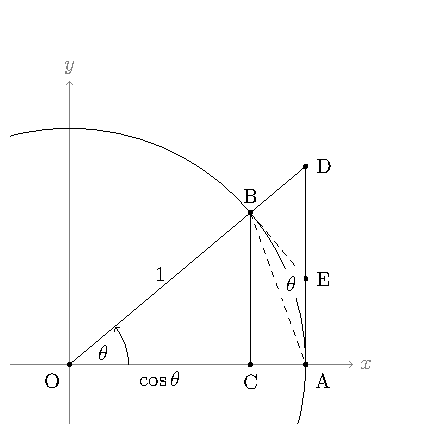
\includegraphics[width=.4\textwidth]{sincx}
\caption{}\label{sinc}
\end{figure}

Let $A$ and $B$ be points of a unit circle with center at $O$ such that $0<\theta<\frac\pi2$ where $\theta$ is the \textit{radian measure} of angle $AOB$. As in Figure \ref{sinc} draw $BC$ perpendicular to $OA$ where $C$ is on $OA$, and draw $AD$ perpendicular to $OA$ where $D$ is on $OB$. In radian measure the angle $\theta$ is defined as the corresponding arc over the radius. Since the radius is $1$ we have
\[
\theta=\frac{\wideparen{AB}}{1},\quad\Rightarrow\quad \wideparen{AB}=\theta
\]
We let "$AB$" stand for the segment $AB$ and also the length of $AB$, and we let "$\wideparen{AB}$" stand for the arc $AB$ and also the length of $\wideparen{AB}$.

\medskip

Consider these statements for $0<\theta<\frac\pi2$.
\begin{enumerate}
  \item $0<BC$ since $B$ and $C$ are distinct points.
  \item $BC=\sin \theta$ by the definition of $\sin \theta$.
  \item $BC<\wideparen{AB}$ because $BC$ is the perpendicular from $B$ to line $OA$ and $\wideparen{AB}$ is not.
\end{enumerate}
Therefore,
\begin{equation}\label{sinc1}
0<\sin\theta<\theta\qquad \mbox{ if } \qquad 0<\theta<\frac\pi2
\end{equation}
Next draw segment $AB$ to form acute triangle $AOB$. Then $0<AB<\theta$ and by the law of cosines,
\[
\overline{AB}^2=1^2+1^2-2\cos \theta.
\]
This implies
\[
\theta^2>2-2\cos\theta
\]
Then
\[
1-\frac{\theta^2}{2}<\cos\theta
\]
Therefore, $\cos\theta<1$ whenever $0<\theta<\frac\pi2$ and
\begin{equation}\label{sinc2}
\theta^2>2-2\cos\theta<1\qquad \mbox{ if } \qquad 0<\theta<\frac\pi2
\end{equation}
Finally, draw $BE$ tangent to circle $O$ at $B$ with $E$ on $AD$. Since two tangents $BE$ and $EA$ could be sides of a polygon circumscribed about circle $O$, then
\[
\overline{AE}+\overline{BE}>\wideparen{AB}
\]
Since $\wideparen{AB}=\theta$,
\[
\theta<\overline{AE}+\overline{BE}.
\]
Since triangle $BED$ is a right triangle with right angle at $B$, then $BE<ED$ and
\[
\overline{AE}+\overline{BE}<\overline{AE}+\overline{ED}
\]
But $\overline{AE}+\overline{ED}=\overline{AD}$ and $AD=\tan \theta$. Therefore,
\begin{equation}\label{sinc3}
0<\theta<\tan \theta\qquad \mbox{ if } \qquad 0<\theta<\frac\pi2
\end{equation}
Now multiply the inequality in (\ref{sinc3}) by $\displaystyle\frac{\cos\theta}{\theta}$ we obtain
\[
0<\cos\theta<\frac{\sin\theta}{\theta}\qquad \mbox{ if } \qquad 0<\theta<\frac\pi2
\]
Bus since $\sin\theta<\theta$ if $0<\theta<\frac\pi2$ by (\ref{sinc1}), then $\displaystyle\frac{\sin\theta}{\theta}<1$ and
\begin{equation}\label{sinc4}
\cos\theta<\frac{\sin\theta}{\theta}<1
\end{equation}
If $-\frac\pi2<\theta<0$, then $0<-\theta<\frac\pi2$ and the statement (\ref{sinc4}) yields
\begin{equation}\label{sinc5}
\cos(-\theta)<\frac{\sin(-\theta)}{-\theta}<1\qquad \mbox{ if } \qquad -\frac\pi2<\theta<0
\end{equation}
But $\cos(-\theta)=\cos(\theta)$ and $\displaystyle\frac{\sin(-\theta)}{-\theta}=\frac{\sin(\theta)}{\theta}$, thus (\ref{sinc4}) and (\ref{sinc5}) combine to yield
\begin{equation}\label{sinc6}
\cos\theta<\frac{\sin\theta}{\theta}<1\qquad \mbox{ if } \qquad 0<|\theta|<\frac\pi2.
\end{equation}
Thus by applying \textit{the squeezing theorem}\footnote{what?} on (\ref{sinc6}) we have
\[
\lim_{\theta\to 0}\frac{\sin(\theta)}{\theta}=1.
\]

\end{document}
